\documentclass[10pt]{article}
\usepackage{amsthm}
\usepackage{amsfonts}
%\usepackage{amsmath}
\usepackage[utf8]{inputenc}
\usepackage{graphicx}
\usepackage{xcolor}
\usepackage[margin=1.0in]{geometry}
\usepackage{fancyvrb}
\usepackage{cprotect}
\usepackage{url}
\usepackage{etoolbox}
\usepackage[hidelinks]{hyperref}
\usepackage[skins,theorems]{tcolorbox}
\usepackage{enumitem}
\usepackage{xcolor}
\usepackage{pifont}
\usepackage{tcolorbox}        % load once, no options
\tcbuselibrary{theorems,skins,breakable} % add features here
%\newcommand*{\vertbar}{\rule[-1ex]{0.5pt}{2.5ex}}
%\newcommand*{\horzbar}{\rule[.5ex]{2.5ex}{0.5pt}}
%\setlist[itemize]{align=parleft,left=1pt..1em}
% \usepackage{tikz}
% \usetikzlibrary{arrows.meta,positioning}
\newcommand{\vertbar}{\,\big|\,}

\usepackage{imakeidx}
\makeindex

\usepackage{listings}
\usepackage{xcolor}

% Define some colors
\definecolor{codegreen}{rgb}{0,0.6,0}
\definecolor{codegray}{rgb}{0.5,0.5,0.5}
\definecolor{codepurple}{rgb}{0.58,0,0.82}
\definecolor{backcolour}{rgb}{0.95,0.95,0.92}

% Define a style
\lstdefinestyle{mystyle}{
    commentstyle=\color{codegreen},
    keywordstyle=\color{blue},
    numberstyle=\tiny\color{codegray},
    stringstyle=\color{codepurple},
    basicstyle=\ttfamily,
    breakatwhitespace=false,
    breaklines=true,
    captionpos=b,
    keepspaces=true,
    numbersep=5pt,
    showspaces=false,
    showstringspaces=false,
    showtabs=false,
    tabsize=4
}

\lstset{style=mystyle}
%\usepackage[T1]{fontenc}
%\usepackage{inconsolata} % optional, nicer monospace font


\usepackage{cmbright}
%\usepackage[OT1]{fontenc}
%\usepackage{helvet}
%\renewcommand{\familydefault}{\sfdefault}

%\usepackage{titlesec}



%\titleformat{\section}
%  {\normalfont\fontsize{14}{17}\sffamily\bfseries}
%  {\thesection}
%  {1em}
%  {}
%
%\titleformat{\subsection}
%  {\normalfont\fontsize{12}{17}\sffamily\slshape}
%  {\thesubsection}
%  {1em}
%  {}



% from https://www.pinterest.co.uk/pin/88664686405122253/
\definecolor{C1}{RGB}{141, 125, 158} %purple
\definecolor{C2}{RGB}{163,156,147} % yellow
\definecolor{C3}{RGB}{99,151,153} % green
\definecolor{C4}{RGB}{195,106,99} % red
\definecolor{C5}{RGB}{124, 132, 128}
\definecolor{C6}{RGB}{67, 69, 75}



\definecolor{Gr}{HTML}{377D71}
\definecolor{Pu}{HTML}{A459D1}
\definecolor{Bl}{HTML}{4D455D}
\definecolor{Te}{HTML}{C1ECE4}
\definecolor{Or}{HTML}{EF6262}
\definecolor{Am}{HTML}{F3AA60}
\definecolor{Co}{HTML}{3C486B}
\definecolor{Wh}{HTML}{FEFBF6}
\definecolor{Ye}{HTML}{FFE196}
\definecolor{Re}{HTML}{E96479}
\definecolor{Pi}{HTML}{FFD0D0}
\definecolor{Rp}{HTML}{FF9EAA}
\definecolor{Wg}{HTML}{EEF3D2}

\newcounter{unit}
\renewcommand{\thesection}{\theunit.\arabic{section}}

\hypersetup{
    colorlinks=false,
    linkcolor=red,
    filecolor=red,      
    urlcolor=red,
    pdftitle={a},
    pdfpagemode=FullScreen,
    }
    
    
 % TCOLORBOX STUFF ----------------------------------------------------------------------------
 

 %  ----------------------------------------------------------------------------
    
%\patchcmd{\section}{\normalfont}{\color{C5}}{}{}
%\patchcmd{\subsection}{\normalfont}{\color{C5}}{}{}


\newcommand{\dfn}[1]{{\underline{#1}}}
\definecolor{sidebarblue}{HTML}{E3F2FD}


\renewcommand{\FancyVerbFormatLine}[1]{\color{gray}{>\,\,#1}}
    
\newtheorem{thm}{Theorem}


\newtheoremstyle{exercise}
{}                % Space above
{}                % Space below
{\color{black}}        % Theorem body font % (default is "\upshape")
{}                % Indent amount
{\bfseries}       % Theorem head font % (default is \mdseries)
{:}               % Punctuation after theorem head % default: no punctuation
{ }               % Space after theorem head
{}                % Theorem head spec
\theoremstyle{exercise}
\newtheorem{exercise}{Exercise}


\newtheoremstyle{example}
  {}                % Space above
  {}                % Space below
  {\color{black}} % Theorem body font (default is "\upshape")
  {}                % Indent amount
  {\bfseries}       % Theorem head font (default is \mdseries)
  {.}               % Punctuation after theorem head (default is no punctuation)
  { }               % Space after theorem head
  {\thmname{#1}\thmnumber{ #2}\thmnote{ \textnormal{(#3)}}}  % Theorem head spec: #1 is name, #2 is number, #3 is note

\theoremstyle{example}
\newtheorem{example}{Example}

% Boxed, breakable 'example' with dashed continuation markers and custom background
	\tcolorboxenvironment{example}{
  enhanced,
  breakable,
  colback=sidebarblue,        % <<< background color
  colframe=black,
  boxrule=1pt,
  arc=5pt,
  left=6pt,right=6pt,top=6pt,bottom=6pt,
  % dashed markers at page breaks
  overlay unbroken={},   % no markers if the box doesn't break
 }

\newtheoremstyle{solution}
{}                % Space above
{}                % Space below
{\color{C5}}        % Theorem body font % (default is "\upshape")
{}                % Indent amount
{\bfseries }       % Theorem head font % (default is \mdseries)
{:}               % Punctuation after theorem head % default: no punctuation
{\newline}               % Space after theorem head
{}                % Theorem head spec
\theoremstyle{solution}
\newtheorem*{solution}{Solution}


\newcommand{\mcS}{\mathcal S}
\newcommand{\mcR}{\mathcal R}
\newcommand{\mcC}{\mathcal C}
\newcommand{\bS}{{\boldsymbol S}}
\newcommand{\bR}{{\boldsymbol R}}
\newcommand{\bC}{{\boldsymbol C}}
\newcommand{\ba}{{\boldsymbol a}}
\newcommand{\bb}{{\boldsymbol b}}
\newcommand{\bs}{{\boldsymbol s}}
\newcommand{\bff}{{\boldsymbol f}}
\newcommand{\br}{{\boldsymbol r}}
\newcommand{\bx}{{\boldsymbol x}}
\newcommand{\bt}{{\boldsymbol t}}
\newcommand{\bv}{{\boldsymbol v}}
\newcommand{\bu}{{\boldsymbol u}}
\newcommand{\bw}{{\boldsymbol w}}
\newcommand{\bc}{{\boldsymbol c}}
\newcommand{\be}{{\boldsymbol e}}
\newcommand{\bq}{{\boldsymbol q}}
\newcommand{\bphi}{{\boldsymbol \phi}}
\newcommand{\brho}{{\boldsymbol \rho}}
\newcommand{\btau}{{\boldsymbol \tau}}
\newcommand{\reals}{\mathbb R}
\newcommand{\ints}{\mathbb N}
\newcommand{\E}{\mathbb E}
\newcommand{\Prob}{\mathbb P}


\newcommand{\sectionrefs}[1]{\par\smallskip\noindent\textbf{References:} #1\par\smallskip}


%%%%%%%%%%%%%%%
% adding space between items
%\usepackage{enumitem}
%\setlist{topsep=1.5em, itemsep=1.1em}





\setcounter{unit}{2}
\setcounter{section}{0}


\begin{document}

\title{Unit 2: Expectation and variance, Normal distribution and CLT}
\author{Ethan Levien}
\maketitle
\tableofcontents



\section*{Introduction}

In this section we introduce expectation. This will help us summarize important properties of the data, such as variance. Then, we will introduce continuous probability distribution (modeling real valued random variables).  The most important is the Normal distribution and discuss its properties. It will be important to understand where the Normal distribution comes from, so we will discuss (in non-rigorous terms) the central limit theorem (CLT).  Time permitted we may also discuss the random walk. 






\section{Expectation, variance and standard deviation}




\subsection{Sample averages and expectation}
\sectionrefs{ \cite[Ch. 3]{evans}}
 Usually it is difficult to obtain the full distribution of a random variable from data and it may not even be that relevant for the questions we are asking. Instead, we would like to summarize properties of a random variable by looking at averages. The simplest example is the \dfn{sample mean}, \dfn{sample average}, or \dfn{empirical average}. 
If $Y_1,Y_2,\dots,Y_n$ are iid samples of $Y$, the sample mean is defined as
\begin{equation*}
\overline{Y} = \frac{1}{n}\sum_{i=1}^nY_i
\end{equation*}
Sometimes the notation $\langle \cdot \rangle$ is used. 
More generally, we might look at the average of some function of a random variable 
\begin{equation*}
\overline{f(Y)} = \frac{1}{n}\sum_{i=1}^nf(Y_i)
\end{equation*}
If we take the function to be 
\begin{equation}
f(y) =1_A(y) =  \left\{\begin{array}{lr} 
1 & \text{if }y \in A\\
0 & \text{if }y \in A
\end{array}\right.
\end{equation}
Then $\overline{f(Y)} \approx P(\{Y \in A\})$, so we can connect the idea of a sample average to estimates of probabilities. Any quantity we compute from data is in some way a sample average, so a great deal of statistics is about understanding the behavior of sample averages. 

A sample average can be computed from the probability distribution.  Suppose each $Y_i$ are random $1,2,3,\dots,m$. If $n$ is large, then the fraction of samples for which $Y_i= y$ will be $P(\{Y_1=y\})$, thus the sample mean converges to the true mean: 
 \begin{equation*}
\overline{Y} =  \frac{1}{n}\sum_{i}Y_i = \frac{1}{n} \sum_{y=1}^m y n_i=\sum_{y=1}^m y \frac{n_i }{n}\approx  \sum_{y=1}^m y P(Y=y)
\end{equation*}
The expression on the right is the definition of the mean, or \dfn{expectation} denoted 
 The expectation is an operation which takes a random variable to a deterministic number and the sample average is the approximate version of this: To summarize
 \begin{equation}\label{eq:EappoverY}
 E[Y] \approx \overline{Y}
 \end{equation}

\begin{example}[Mean and variance of Bernoulli random variable]
Let $Y$ be a Bernoulli random variable with parameter $q$. We will use the convention that $Y=1$ with probability $q$.\\


\noindent
\underline{Question}: What is $E[Y]$ and ${\rm var}(Y)$?\\

\noindent
\underline{Solution}: Using the definitions above
\begin{equation*}
E[Y] = P(Y=0)\times 0 + P(Y=1)\times 1 = q
\end{equation*}
similarly you should be able to see that ${\rm var}(Y) = q(1-q)$. 
In the python notebook we test the formula $E[Y]=q$. 
\end{example}


Based on this example, we can see that to estimate $q$ we can use $\hat{q} = \bar{Y}$ (as expected). Here I'm defining $\hat{q}$ as shorthand for an estimator of $q$. 


\subsection{Measuring variation}
 In many cases we would like to measure deviations from the mean. For this we define \dfn{variance},
\begin{equation*}
{\rm var}(Y) = E[(Y-E[Y])^2]
\end{equation*}
Another way to write this is 
\begin{equation*}
 {\rm var}(Y) = E[Y^2] - 2E[Y]^2 + E[Y]^2 = E[Y^2]-E[Y]^2
\end{equation*}
We can of course estimate this from a large number of samples, although as we will later see the obvious way of doing this by replacing the expectations with sample averages is, perhaps surprisingly, not the best approach (it is biased estimator). To measure ``how much variation'' there is in a random variable, we need to compare the variance to the mean. However, these is a problem with doing this directly: the variance has different units than the mean. For example, say we are looking at human height. If the mean height is about $170 \,\text{cm}$, then the variance might be something like $100 \,\text{cm}^2$. This is hard to interpret because the mean is measured in centimeters, while the variance is in squared centimeters. To make the comparison meaningful, we first take the square root of the variance to obtain the \dfn{standard deviation}, which brings the measure of spread back into the same units as the mean (in this case, centimeters). Now we can meaningfully say that the spread around the mean height is about $10 \,\text{cm}$.  

But even the standard deviation is not enough by itself when we want to compare variability across different contexts. Suppose we measure the weights of the same individuals, where the mean is around $70 \,\text{kg}$ and the standard deviation is $10 \,\text{kg}$. The ``10'' here is not directly comparable to the ``10'' cm in height, because the scales of measurement are different. What matters is not the absolute size of the variation, but its size \emph{relative to the mean}.  

This leads us to the \dfn{coefficient of variation (CV)}, defined as 
\begin{equation}
\text{CV} = \frac{\sigma}{\mu},
\end{equation}
where $\sigma$ is the standard deviation and $\mu$ is the mean. The CV is unitless and therefore allows for comparisons across variables measured in different units or across distributions with very different scales. For example, a CV of $0.06$ in human height ($10/170$) indicates less relative variability than a CV of $0.14$ in weight ($10/70$).  

Thus, the CV is the correct measure of variation when our goal is to compare variability across different contexts, because it removes dependence on units and scale while still preserving the intuitive meaning of variation as ``spread relative to the average.''  




\subsection{Conditional expectation}
\sectionrefs{\cite[Ch. 1 Sec. 2 and Ch. 2.1]{evans}}

 We define the conditional expectation  \cite[Definition 3.5.1]{evans} as the expectation of the conditional variable; that is, 
\begin{equation*}
\E[X|Y=y] = \sum_{x} xP(X|Y=y)
\end{equation*}
With samples
\begin{equation*}
\{(x_1,y_1),\dots,(x_n,y_n)\}
\end{equation*}
 we could obtain this from a sample by taking the sample mean of $X$ among just the samples where $y_i = y$; that is, let 
 \begin{equation*}
 n_1 = \text{number of samples where $y_i = y$}
 \end{equation*}
 then 
 \begin{equation*}
 \E[X|Y=y] \approx  \frac{1}{n_1}\sum_{i=1}^n1_{\{y_i = y\}}x_i
 \end{equation*}
 where $1_{\{y_i = y\}}$ is the \dfn{indicator function}
 \begin{equation*}
 1_{\{y_i = y\}} = \left\{ \begin{array}{cc}
 0 & \text{ if } y_i\ne y\\
  1 & \text{ if } y_i=y
  \end{array}\right.
 \end{equation*}
 As we already noted, the conditional probabilities can tell us whether two variables are independent. That is, $P(X|Y) = P(X)$ if and only if $X$ and $Y$ are independent. If $X$ and $Y$ are independent, then $E[X|Y=y]= E[X]$ for all $y$ but the converse is false: {\bf it is possible that this is true but $X$ and $Y$ are not independent!} We will say about this later.  




\begin{example}[Computing conditional expectation]
Consider the pair of random variables $(Y_A,Y_B)$ defined by the probability distribution we saw in week 1:
\begin{equation}\label{eq:gene}
P(Y_A,Y_B) = \left\{ \begin{array}{cc}
1/2 & \text{ if }Y_A=0 \text{ and } Y_B = 0\\
1/8 & \text{ if }Y_A=0 \text{ and } Y_B = 1\\
1/8 & \text{ if }Y_A=1 \text{ and } Y_B = 0\\
1/4 & \text{ if }Y_A=1 \text{ and } Y_B = 1\\
\end{array}
 \right.\\
\end{equation}


\noindent
\underline{Question}: Compute $E[Y_A|Y_B=1]$\\

\noindent
\underline{Solution}: We can obtain the conditional distribution of $Y_A$ as 
\begin{equation*}
P(Y_A=1|Y_B = 1) = \frac{P(Y_A=1,Y_B=1)}{P(Y_B=1)} = \frac{1/4}{3/8} = \frac{2}{3}
\end{equation*}
Note that his means $P(Y_A=0|Y_B = 1) = 1/3$ and so the conditional distribution of  $Y_A$ is 
\begin{equation*}
Y_A|(Y_B=1) \sim {\rm Bernoulli}(2/3)
\end{equation*}
which means 
\begin{equation*}
E[Y_A|Y_B=1] = \frac{2}{3}.
\end{equation*}

\end{example}

\begin{example}[Computing conditional expectation from data ]
Consider the following data containing children's test scores and some other information. 
\begin{lstlisting}[language=Python]
# Here is some data on children's test scores
url = (
    "https://raw.githubusercontent.com/"
    "avehtari/ROS-Examples/"
    "master/KidIQ/data/kidiq.csv"
)
df = pd.read_csv(url)
df
\end{lstlisting}

Let $Y$ be the test score and $X$ be a binary variable representing whether the mother graduated high school.\\

% Supp
%\begin{align*}
%X &\sim {Bernoulli}(q)\\
%Y|(X=x) &\sim {\mr Normal}(\mu_1 X + \mu_2 (1-x),\sigma)
%\end{align*}

\noindent
\underline{Question}: Compute $E[Y|X=0]$ and $E[Y]$. Do you think $X$ and $Y$ are independent? \\

\noindent
\underline{Solution}: See Python notebook.



\end{example}




  \subsection{Properties of expectation}\label{prop:lin} 
  
  Previously, I introduced the notation of expectation and we saw how to compute expectations in Python. Now we cover some addition properties. 
  \begin{enumerate}
  \item {\bf Linearity  \cite[Theorem 3.1.2]{evans}:} For two random variables $X$ and $Y$ with discrete samples spaces $S_X$ and $S_Y$, 
  \begin{equation*}
  E[X+Y] = E[X]+E[Y]
  \end{equation*}
  \begin{proof} We have 
  \begin{align*}
  E[X+Y] &= \sum_{y \in S_Y}\sum_{x\in S_X} (x+y)P(X=x,Y=y) \\
  &= \sum_{x \in S_X} \sum_{y \in S_Y} xP(X=x,Y=y)  +  \sum_{x \in S_X} \sum_{y \in S_Y} yP(X=x,Y=y) \\
  &= \sum_{x \in S_X} x\left( \sum_{y \in S_Y}P(X=x,Y=y)  \right)+   \sum_{y \in S_Y} y\left( \sum_{x \in S_X} P(X=x,Y=y)\right) \\
  &= E[X] + E[Y]
  \end{align*}
  \end{proof}
    \item {\bf Multiplication by a constant \cite[Theorem 3.1.2]{evans}:} If $a$ is a constant (meaning it is not random), then 
    \begin{equation*}
      E[aX] =  a E[X]
    \end{equation*}
     \begin{proof}  Left as an exercise. 
     \end{proof}
  \item \label{prop:ind}  {\bf Factoring for independent variables \cite[Theorem 3.1.3]{evans}:} If $X$ and $Y$ are independent, the 
  \begin{equation*}
  E[XY]=E[X]E[Y]
  \end{equation*}
    \begin{proof} Using independence, we have 
    \begin{align*}
     E[XY] &= \sum_{x \in S_X}\sum_{y \in S_Y} xy P(X=x,Y=y)  \\
     &= \sum_{x \in S_X}\sum_{y \in S_Y} xP(X=x)yP(Y=y) \\
     &= \left( \sum_{x \in S_X} xP(X=x)\right)\left( \sum_{y \in S_Y} yP(X=x)\right)= E[X]E[Y]
    \end{align*}
    \end{proof}
    \item {\bf Tower property \cite[Theorem 3.5.2]{evans}:} Let $X$ and $Y$ be two random variables,  
   \begin{equation*}
   E[E[X|Y]] = E[X]
   \end{equation*}
   where by $E[X|Y]$ we mean the random variable constructed by taking the conditional expectation of $X$ given a random value of $Y$. Another way to define this is to introduce the deterministic function  $f(y) = E[X|Y=y]$ which outputs a number for every value $y \in Y$. Then we define the random variable $E[X|Y] = u(Y)$.  Therefore
   \begin{equation*}
   E[E[X|Y]]  = E[f(Y)] 
   \end{equation*}
   \begin{proof}
   Left as an exercise. 
   \end{proof}
  \end{enumerate}

  
  
   \begin{example}[Calculating probabilities]
Consider the model probability model for a variable $X$ (similar to Equation \ref{eq:gene}) 
\begin{equation*}\label{eq:gene}
P(X) = \left\{ \begin{array}{cc}
1/2 & \text{ if }X=1\\
1/8 & \text{ if }X=2\\
1/8 & \text{ if }X=3\\
1/4 & \text{ if }X=4
\end{array}
 \right.\\
 \end{equation*}
 and define 
 \begin{equation*}
 Y = X\cdot Z,\quad Z = {\rm Geometric}(1/2). 
 \end{equation*}
In this example we consider the joint distribution $(Y,X)$. \\


\noindent
\underline{Question}: Using simulations of this model, illustrate properties of expectation in Python.\\

\noindent
\underline{Solution}: See Python notebook. The one that requires the most explanation is the tower property.
We will use simulations to show. Let $(X_1,Y_2),\dots,(X_N,Y_N)$ be our samples. We will show that $E[X] = E[E[X|Y]]$. The left hand side is easy to approximate with samples -- just take the mean of the $X$ values. To compute $E[X|Y]$ we need to compute $E[X|Y=y]$ for each $y$. If $n_y$ is the number of samples such that $Y_i=y$ then 
\begin{equation*}
E[X|Y=y] \approx \frac{1}{n_y}\sum_{\{i:Y_i =y\}}X_i
\end{equation*}
The sum is over all the $Y_i$ for which $Y_i=y$. We could also write this sum as $\sum_{i=1}^NX_i1_{Y_i=y}$. 
This means 
\begin{equation*}
E[E[X|Y]] \approx E\left[ \frac{1}{n_y}\sum_{\{i:Y_i =Y\}}X_i  \right] = \sum_{y \in S_y}P(Y=y)\underbrace{\left(\frac{1}{n_y}\sum_{\{i:Y_i =y\}}X_i  \right)}_{\approx E[X|Y=y]}
\end{equation*}
Now use that $P(Y=y) \approx n_y/N$, therefore 
\begin{equation*}
E[E[X|Y]]  \approx \sum_{y \in S_y}\frac{1}{n_y}\sum_{\{i:Y_i =y\}}X_i  \frac{n_y}{N}
\end{equation*}
Notice that when we cancel the $n_y$ terms we just get the usual sample mean of $X$: 
\begin{equation*}
E[E[X|Y]]  \approx \frac{1}{N} \sum_{y \in S_y}\sum_{\{i:Y_i =y\}}X_i   =  \frac{1}{N}\sum_{i=1}^NX_i = \overline{X} \approx E[X]
\end{equation*}

 \end{example}

% \begin{example}[Binomial distribution in python]
% Let's explore binomial random variables in python. 
% \end{example}
 
\begin{example}[Expectation of binomial]\label{ex:binomial_stats}
Let $Y$ be a binomial random variable. \\
 
 \noindent
\underline{Question:} What are $E[Y]$ and ${\rm var}(Y)$?\\
 
 
  \noindent
\underline{Solution:} 
\begin{equation*}
E[Y] = \sum_{k=1}^N k P(Y=k) =\sum_{k=1}^N k  {N \choose k}q^{k}(1-q)^{N-k} = \cdots. 
\end{equation*}
A much easier way is to use the definition of a Binomial random variable and exceptions 
\begin{align*}
E[Y] &= E\left[\sum_{j=1}^NX_i\right]\\
& \underset{(1)}{=}  \sum_{j=1}^NE\left[X_i\right]  =Nq
\end{align*}
where we are using the fact that averages are additive (property (1)). Similarly, 
\begin{align*}
E[Y^2] &= E\left[\left(\sum_{j=1}^NX_i\right)^2\right] = E\left[\sum_{i=1}^N\sum_{j=1}^NX_iX_j\right] \\
&\underset{(1)}{=}  \sum_{i=1}^N\sum_{j=1}^NE[X_iX_j]\underset{(3)}{=} \sum_{i=1}^N\sum_{j \ne i}^Nq^2 +  Nq(1-q) + Nq^2\\
&= N(N-1)q^2 + Nq(1-q)  +  Nq^2 = Nq(1-q)  + N^2q^2
\end{align*}
Therefore 
\begin{equation*}
{\rm var}(Y) =E[Y^2]-E[Y]^2 =  Nq(1-q)
\end{equation*}
\end{example}
 
To summarize what we learned in Example \ref{ex:binomial_stats}
\begin{equation}\label{eq:binomial_meanvar}
E[Y] = qN \quad\quad{\rm var}(Y) = Nq(1-q). 
\end{equation}


 
 The important observation that the mean grows much faster with $N$ than the variance is also captured by the coefficient of variation: 
\begin{equation*}
{\rm CV} = \frac{\sqrt{{\rm var}(Y)}}{\E[Y]} = \sqrt{\frac{(1-q)}{q} \frac{1}{N}}. 
\end{equation*}
The idea is that we are measuring the variation \emph{relative} to the average. This is relevant for many applications where we only care about the relative deviations. 

%\item 
% Binomial samples can be generated in numpy with
% \begin{Verbatim}
%y = np.random.binomial(n,p,n_samples)
% \end{Verbatim}
 %\item Often we are interested not in $Y$, but the fraction $\phi = Y/N$. For example, we might be interested in the vote share in an election. 
 
 \begin{example}[Election modeling]
 Consider a model of votes in an election involving two candidate. Let $q$ be the fraction of people in the population who support candidate one and suppose $N$ people vote at the election (you can assume $N$ is much less than the total number of people in the population, as voter turnout is low). Then the number of people, $M$, who vote for the first candidate can be modeled as 
\begin{equation*}
M \sim {\rm Binomial}(N,q)
\end{equation*}
Think about the assumption we are making when we use this model. \\

 \noindent
\underline{Question:} Suppose there is a city in which a fraction $q = 0.51$ of people support a candidate for city council. If $N=1000$ people turnout for the election, what is the chance that the actual vote share, $\phi = M/N$, differs from the actual fraction of support throughout the population by more than $1\%$?\\

 \noindent
\underline{Solution:} See the Python notebook.
\end{example}

 In the problem above the vote share is the same as the sample mean:
\begin{equation*}
\overline{X_i} = \frac{M}{N} =  \frac{1}{N}\sum_{i=1}^NX_i
\end{equation*}
You should be able to see that $E[\phi] = q$. What about the variance? 
 \begin{equation*}
{\rm var}(\phi) = {\rm var}(Y/N) = \frac{1}{N^2}{\rm var}(Y) = \frac{q(1-q)}{N}
 \end{equation*}
 Notice that this will tend towards zero as $N \to \infty$. Meanwhile, $E[\phi]$ has no dependence on $N$. This is a consequence of the fact that the CV is decreasing with $N$ and it allows us to determine $q$ by approximating $E[\phi]$ with the sample mean.








 \section{Asymptotic probabilities: LLN and CLT}
 The goal of this section is to understand the distribution of a sum of iid random variables when $N$ is large. This is obviously relevant if we want to be more precise about how accurate our estimates are. We begin with the law of large numbers, which simply makes Eq. \ref{eq:EappoverY} -- the statement that the sample average approximates the expectation -- precise. 
 
 \subsection{LLN}
The binomial distribution illustrates a very basically principle that we have already used a number of times: When we sum over a large number of independent random variables and divide by the total number, the result is close to the mean. This is the Law of Large Numbers (LLN). 
 \begin{thm}[Law of Large numbers] Let $X_i$ be independent and identically distributed and set
 \begin{equation*}
 S_N = \sum_{i=1}^N X_i.
 \end{equation*}
 If $E[X_i]<\infty$, then $S_N/N \to E[X_i]$. 
 \end{thm}
 This is not very precise, since we should really be specific about what it means for a random number to converge to something, but for our purposes it will suffice to think of this as saying that for large enough $N$, $S_N/N$ will not differ from $E[X_i]$ very much. See  \cite[Theorem 4.2.1]{evans} for a more technical statement. Another way to say this is that for iid random variables $X_i$, $i=1,\dots,N$, the sample average $\overline{X}$ approach $E[X_i]$. 
The binomial distribution actually tell us more, it tell us that the variation around $E[X_i]$ is proportional to $1/\sqrt{N}$. It is natural to ask whether this is also true for other random variables. The key is that the dependence on $N$ in Equations \ref{eq:binomial_meanvar} does not depend on the distribution of $X_i$! So if $X_i$ is the roll of a dice, or a geometric distribution, we expect the same thing to hold. 
%  \begin{thm}[prerequisite to CLT] Let $X_i$ be independent and identically distributed with $E[X_i] = \mu_x<\infty$ and ${\rm var}(X_i) = \sigma_x^2<\infty$ $\sqrt{{\rm var}(S_N/N) }= \sigma_x/\sqrt{N}$. 
% \end{thm}
The behavior of random sums is in-fact even more universal than this argument suggests. We can actually describe the distribution of any\footnote{With the caveat that here we only deal with the case where ${\rm var}(X_i)<\infty$} random sum with a single distribution.  In order to describe this distribution, we need to introduce the notion of continuous random variables. 

 \subsection{Continuous probability distributions}
To describe what happens to the distribution of the sum, we need to explain how to model continuous probability distributions. This is because when taking a sample average over a very large number of iid variables, $\overline{Y} = \sum_{i=1}^n Y_i/n$, even if $Y_i$ can only take a finite number of values (say it's Bernoulli), the sample average can take an increasing large number of values as $n$ becomes large. This was seen with the Binomial distribution, were we begin with Bernoulli random variables and obtain a random variable which can take values in the sample space $\{0,1/N,2/N,\dots,1\}$. As $N \to \infty$ the sample space becomes the interval $[0,1]$, but the theory of such probability distribution is not covered by our discussion so far. Fortunately, most of what we learned will carry over! Basically, you just need to replace sums with integrals, and I will never ask you to evaluate integrals in this course.  

Let's start by introducing a new random variable,  
 \begin{equation*}
 Y \sim {\rm Uniform}(a,b).
 \end{equation*}
This means an equal chance of taking any number in the interval $[a,b]$ (we assume $a<b$). Let $L=b-a$. This is distinct from other distributions we have encountered in that it is a \dfn{continuous distribution}.  For the uniform distribution, 
 \begin{equation*}
 P(y_1\le Y \le y_2) = \frac{y_2-y_1}{L}
 \end{equation*}
 for $a<y_1<y_2<b$. 
 That is, the chance for $Y$ to fall in any interval is simply the length of that interval. This insures that that the probability of $Y$ being somewhere in $[a,b]$ is one: $P(a\le Y\le b) = 1$. Note that as $y_2 \to y_1$, $P(y_1\le Y \le y_2) \to 0$. This tells us that the chance for $Y$ to take any specific value is $0$. Indeed, there are simply two many number (uncountably many) in any interval to assign positive probability to each.
 
 For continuous variables, it is sometimes useful to work with the density, $f(y)$ (we will use lower case letters for density and uppercase for probability distributions).The density $f(y)$ of a continuous random variable is a positive function such that 
\begin{equation*}
P(a<X<b) = \text{area under $f(y)$ between $a$ and $b$} = \int_a^bf(y)dy
\end{equation*}
We can think of $f(y)$ as the the probability per unit $Y$, meaning that if we look in a small interval 
 \begin{equation*}
f(y)dy = P(y \le Y \le y+dy) = \frac{dy}{L}.
 \end{equation*}
 Thus, for uniform distribution the density is $1/L$ if $y \in [a,b]$ and $0$ otherwise.  Note the following properties of $f(y)$
 \begin{enumerate}
 \item It is positive
 \item The area under $f(y)$ is one (this is the continuous version of the condition that discrete probability distributions must sum to one). 
 \end{enumerate}


\begin{figure}[h]
\centering
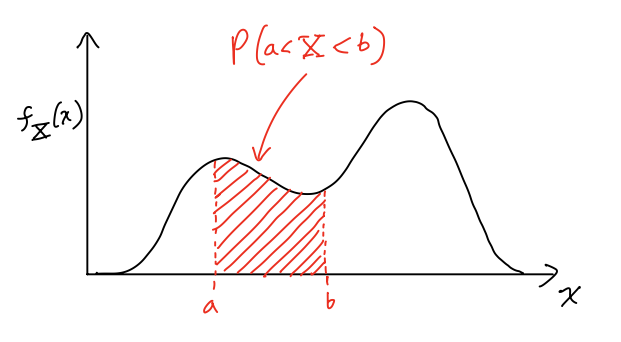
\includegraphics[width=0.6\textwidth]{./../figures/density}
\caption{The density and its relationship to probabilities}\label{fig:density}
\end{figure}



\begin{example}[Condition with continuous random variables]
If $Y$ is uniform on $[0,1]$. \\


\noindent
\underline{Question:}  What is the density of $Y|(Y<1/2)$? Check the answer with simulations.\\

 \noindent
\underline{Solution:} We can start with the definition of density
\begin{align*}
P(y_1<Y<y_2|Y<1/2) &= \frac{P(y_1<Y<y_2,Y<1/2)}{P(Y<1/2)}
\end{align*}
What is the think on the top? We will assume $y_1>0$ and $y_2<1/2$, then the numerator is $y_2-y_1$, since $Y<1/2$. The key here is that if $Y \in [y_1,y_2]$ $Y<1/2$ is automatically true, so the chance that BOTH of these things are true in a sample is the chance that the more restrictive one is true.

The denominator is $P(Y<1/2) = 1/2$. This means
\begin{equation*}
P(y_1<Y<y_2|Y<1/2) = 2(y_2-y_1)
\end{equation*}
This means the density is
\begin{equation*}
f(y|Y<1/2) = 2
\end{equation*}
Thus
\begin{equation*}
Y|(Y<1/2) \sim {\rm Uniform}(0,1/2)
\end{equation*}
We also check this with simulations in the Python notebook. 
\end{example}


  \subsection{The Gaussian curve}
We know meet the most important probability model of all. This is the Normal distribution, which has a density 
   \begin{equation*}
   f(x) = \frac{1}{\sqrt{2\pi \sigma^2}}e^{-\frac{(x-\mu)^2}{2 \sigma^2}}
   \end{equation*}
 Despite the simplicity of the density function, calculating probabilities for Normal random variable by computing the area under the curve (integrating) is difficult. Instead we can remember some rough estimates based on the following figure. 

\begin{figure}[h]
\centering
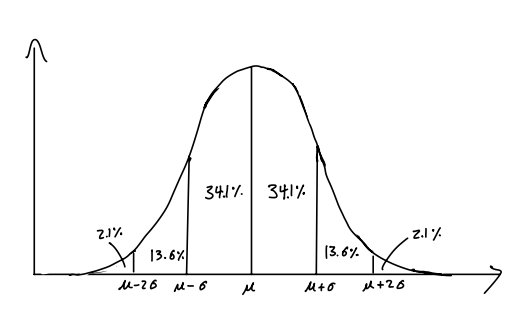
\includegraphics[width=0.6\textwidth]{./../figures/bellcurve}
\caption{Probabilities in the Normal distribution}\label{fig:bellcurve}
\end{figure}



\begin{example}[Calculating probabilities for Normal distribution]
 We use the curve above to calculate probabilities of events in the Normal distribution. Suppose
\begin{equation*}
Y \sim {\rm Normal}(5,4)\\
\end{equation*}


 \noindent
\underline{Question:} What is (approximately) $P(Y > 7)$? \\

 \noindent
\underline{Solution:} Note that $5 + 2 =  7$, so this is asking how likely it is that a Normal variable is greater than $1$ standard deviation above the mean. This about $13.5+2 = 15.5\%$. We can always easily compute these probabilities in python as well.\\ 



 \noindent
\underline{Question:} What is
\begin{equation*}
P(Y>3|Y<7)?
\end{equation*}

 \noindent
\underline{Solution:} In this case we would use
\begin{equation*}
P(Y>3|Y<7) = \frac{P(Y>3,Y<7)}{P(Y<7)} 
\end{equation*}
Notice that $3 = 5-2 = \mu-\sigma$ and we already saw $7 = 5+2 = \mu+\sigma$, so $P(Y<7) \approx 0.839$ and $P(Y>3,Y<7) \approx 0.682$, thus the result is about $0.81$. 



\end{example}



  
  \subsection{The central limit theorem and sample distribution}
  
  
 We now have the formalism in place to state the Central Limit Theorem (CLT) in more precise terms. 
 \begin{thm} Let $X_i$ be a sequence of iid random variables and let 
 \begin{equation*}
E[X_i] = \mu,\quad  {\rm var}(X_i) = \sigma^2
 \end{equation*}
  and set 
  \begin{equation*}
 S_N = \sum_{i=1}^N X_i.
 \end{equation*}
 Then 
 \begin{equation}\label{eq:clt}
P\left( \frac{S_N-N\mu}{\sqrt{N \sigma^2}}<z\right) \to P(Z<z) 
 \end{equation}
Where
\begin{equation*}
Z \sim {\rm Normal}(0,1)
\end{equation*}
 \end{thm}
 The normal variable $Z$ with zero mean and variance one is called a \dfn{standard normal} random variable. Since evaluations of the CDF of a standard normal random variable appear so often, we use the shorthand 
 \begin{equation*}
 \Phi(z) = P(Z<z).
 \end{equation*}

 
\begin{example}[Binomial] Let 
\begin{equation*}
Y \sim {\rm Binomial}(N,q)
\end{equation*}


 \noindent
\underline{Question:} Assume $N$ is even and use the central limit theorem to approximate $P(Y<N/2)$ with a Normal distribution. How does the accuracy depend on $N$ and $q$? \\

 \noindent
\underline{Solution:} Using that $\mu = E[X_i] = q$ and $\sigma^2 = {\rm var}(X_i) = q(1-q)$, we find that the normal approximation to $Y$ is 
\begin{equation*}
P\left( \frac{Y - Nq}{\sqrt{N \sigma^2}} <z\right) \to P(Z<z)
\end{equation*}
for 
\begin{equation*}
Z \sim {\rm Normal}(0,1). 
\end{equation*}

Now we write
\begin{align*}
P\left( Y<N/2\right) &= P\left(Y - Nq <N/2-Nq\right) \\
&= P\left(\frac{Y - Nq}{\sqrt{N q(1-q)}} <\frac{N/2-Nq}{\sqrt{N q(1-q)}}\right)\\
&= P\left(\frac{Y - Nq}{\sqrt{N q(1-q)}} < \sqrt{N} \frac{1-2q}{2\sqrt{q(1-q)}}\right)\\
&\to P\left(Z < \sqrt{N} \frac{1-2q}{2\sqrt{q(1-q)}}\right) = \Phi\left( \sqrt{N} \frac{1-2q}{2\sqrt{q(1-q)}}\right)
\end{align*}
We can compute this in Python, both by generating samples and using the CDF function.  

\begin{lstlisting}[language=Python]
import numpy as np
from scipy.stats import norm, binom

# parameters
N, q = 200, 0.3
trials = 100000

# exact probability via binomial CDF
exact = binom.cdf(N//2 - 1, N, q)

# CLT approximation using Normal CDF (no continuity correction)
z = np.sqrt(N) * (1 - 2*q) / (2 * np.sqrt(q * (1 - q)))
clt_approx = norm.cdf(z)

# Monte Carlo estimate
samples = np.random.binomial(N, q, size=trials)
mc_estimate = np.mean(samples < N/2)

print(f"Exact:       {exact:.4f}")
print(f"CLT approx:  {clt_approx:.4f}")
print(f"Monte Carlo: {mc_estimate:.4f}")
\end{lstlisting}


\end{example}



 {\bf Note on iid assumption:} One of the most important things to recognize about the CLT when it comes to application is that the assumptions that the $X_i$ are independent are not that important, so long as they are not too correlated. Even though the precise quantitive statement of the CLT won't when there are correlations, the sum will still be well approximated by a Normal distribution. 






\subsection{Properties of Normal random variables}

 {\bf Linear transformations of Normal random variables:}  Suppose 
\begin{equation*}
Z \sim {\rm Normal}(0,1)
\end{equation*}
and define 
\begin{equation*}
X = \sigma Z + \mu 
\end{equation*}
Then 
\begin{align*}
P(X<x) &= P(\mu + \sigma Z<x) \\
&= P\left(Z<\frac{x - \mu}{\sigma}\right)
%&= \int_0^{\frac{x - \mu}{\sigma}}f(x)dx
\end{align*}
Hence 
\begin{equation*}
X \sim {\rm Normal}(\mu,\sigma^2).
\end{equation*} 
With this understanding of how to linearly transform a Normal random variable, we can see that the CLT can be informally stated as
\begin{equation*}
S_N \approx S_{\rm CLT} \sim {\rm Normal}(N\mu,N\sigma^2)
\end{equation*}
 More generally, 
\begin{equation*}
X \sim {\rm Normal}(\mu_x,\sigma_x)
\end{equation*}
Now consider 
\begin{equation*}\label{eq:linear}
Y = aX + b 
\end{equation*}
At this point it should make sense that $Y$ is also normal. 
 but what are the mean and variance? Taking the average of both sides, 
\begin{equation*}
E[Y] = a\mu + b
\end{equation*}
and 
\begin{equation*}
{\rm var}(Y) = {\rm var}(aX) + {\rm var}(b)
\end{equation*}
Form the formula for variance, we know ${\rm var}(aX)  = a^2{\rm var}(X)$. Also, ${\rm var}(b) =0$
So 
\begin{equation*}\label{eq:normal_linear_trans}
Y \sim {\rm Normal}(a\mu_x + b,a^2\sigma_x^2).
\end{equation*}
Note that in going from $Z$ to $X$ and $X$ to $Y$, we are just multiplying and shifting everything.
Think about what this does to the histogram. 
 The process of going from $X$ to $Z$ is called standardizing. For any variable $X$ the \dfn{standardized} variable is defined as 
\begin{equation*}
Z = \frac{X-\mu_x}{\sigma_x}
\end{equation*}
 {\bf Transforming $X$ to a standard Normal is equivalent to measuring $X$ in units of standard deviations.} For example, if we make a histogram of $X$, all this transformation does is change the $X$ axis to units of standard deviations from the mean. 

  \begin{thm}[Special case of Theorem 4.6.1 in \cite{tabak}]\label{thm:addingnormal}
Let
\begin{align*}
X_1 &\sim {\rm Normal}(\mu_1,\sigma_1^2)\\
X_2 &\sim {\rm Normal}(\mu_2,\sigma_2^2)
\end{align*}
be independent, then 
\begin{equation*}
aX_1+bX_2 + d \sim {\rm Normal}\left(a\mu_1+b\mu_2+d,a^2\sigma_1^2 + b^2\sigma_2^2\right)
\end{equation*}
 \end{thm}



\newpage

\section*{Exercises}

 % ------------------------------------------------------------------------------------------------------------------------------------------
\begin{exercise}[Computing conditional averages \ding{111}]
Suppose we have some data representing samples of a pair of random variables $(Y_1,Y_2)$: 
\begin{equation*}
\{(1,2),(1,2),(3,1),(1,4),(3,3),(2,2),(1,5)\}
\end{equation*}
Compute the following both by hand and with Python. 
\begin{enumerate}[label=(\alph*)]
\item $E[Y_1]$
\item $E[Y_1|Y_2=2]$
\item $E[Y_2|Y_1=1]$
\item $E[Y_2|Y_1>1]$
\end{enumerate}
\end{exercise}

\begin{exercise}[\ding{111}]
Do Exercises 3.1.3, 3.1.4, 3.1.10, 3.1.14  in  \cite{evans} and for each one check your answer using simulations. 
\end{exercise}

 % ------------------------------------------------------------------------------------------------------------------------------------------
\begin{exercise}[Independence and conditional expectation \ding{111}]
Let $X$ and $Y$ be two random variables with (discrete) sample spaces $S_X$ and $S_Y$.  (you can find these in the textbook, but give them a try yourself first). 
\begin{enumerate}[label=(\alph*)]
\item Show that if $X$ and $Y$ are independent $\E[X|Y=y]=\E[X]$ and $\E[Y|X=x]=\E[Y]$ for all $x \in S_X$ and $y \in S_Y$.  You may assume $S_X$ and $S_Y$ have a finite number of elements, e.g. $S_X = \{1,2,3,4\}$. 
\item Prove the tower property of expectation, which says that 
\begin{equation*}
\E[X] = \sum_{y \in S_Y}\E[X|Y=y]P(Y=y)
\end{equation*} 
This is sometimes stated as $\E[X] = \E[\E[X|Y]]$ where the inner expectation is interpreted as a random variable depending on the value of $Y$. 
\item Show that if $X$ and $Y$ are independent, then 
\begin{equation*}
{\rm var}(X+Y) = {\rm var}(X) + {\rm var}(Y)
\end{equation*} 

%\item Similar to how we define conditional expectation, we can define the conditional variance
%\begin{equation*}
%{\rm var}(X|Y=y) = \sum_{x\in S_X}(x-\E[X|Y=y])^2P(X=x|Y=y)
%\end{equation*}
%In general, do you think that conditioning will make the variance greater or less than the original variance of $X$?  Try to come up with an answer based solely on the intuitive definition of variance and conditioning, rather than using formulas and theorems. Feel free to test your answer with math or simulations though. 
\end{enumerate}
\end{exercise}





%\begin{exercise}[A first taste of hypothesis testing]
%Last spring, $1425$ out of  $2748$ of student voted ``I have no confidence in President Beilock's leadership'', which comes out to $51.86\%$. 
% Let's try to understand if this small margin could be a reflection of randomness in who voted rather than a true reflection of the student body's preference. To answer this, we make the \emph{null hypothesis} that in reality exactly $1/2$ of the  $6300$ students at Dartmouth support the vote of no confidence. We can then view the $2748$ students who voted as random samples from this pool of students. Under the null hypothesis, how likely is the vote margin to be as large as it was in reality?  You may ignore the chance that we could in principle sample the same student twice and you can either use simulations or formulas. 
%\end{exercise}





\begin{exercise}[Conditioning with continuous variables \ding{111}] Let
\begin{align*}
Z_1 &\sim {\rm Normal}(0,1)\\
Z_2 &\sim {\rm Normal}(1,2)
\end{align*} 
Compute each of the following using Python
\begin{enumerate}[label=(\alph*)]
\item $P(Z_1 + Z_2>3)$
\item $P(Z_1 + Z_2>3|Z_1<-1)$
\item $P(Z_2Z_1>0|Z_1+Z_2<4)$
\end{enumerate}
\end{exercise}


\begin{exercise}
Do Exercise  2.4.2 in  \cite{evans} using simulations. You can also check your answer using calculus if you wish. 
\end{exercise}

\begin{exercise}
The {\bf random walk} is a foundational model in nearly every area of science.  It describes the "motion" of a variable which moves randomly over time without any memory of its past. Einstein developed a theory of the motion of microscopic particles based on random walks and they have been used as rudimentary models of stock prices. 

We can define a random walk as follows. 
Let $X_0=0$ and define $X_k$ for $k=1,2,3,\dots$ by the recursive formula 
\begin{align}\label{eq:rw}
X_{k+1} = X_{k}  + \Delta(2U_k - 1)
\end{align}
where $\Delta$ is a constant and 
\begin{equation*}
U_k  \sim {\rm Bernoulli}(1/2)
\end{equation*}
are iid random variables. 


We can think of $X_k$ as the position of a person who is randomly walking with 50-50 chance of the moving to the left or right by $\Delta$ at each time-step. The entire sequence $X_0,X_1,X_2,\dots$ is referred to as the path of the random walker. 
\begin{enumerate}[label=(\alph*)]
\item Write a python function simulaterw(Delta,K) which simulates a random walk for $N$ steps. Yours code should return the entire path in a numpy array. Make some plots of $X_k$ vs. $k$. 
\item What are $E[X_k|X_{k-1}=2]$ and $E[X_k]$? 
%\item A much harder problem is to calculate $E[X_k|X_{k-1}>0]$. Don't calculate it, but explain why this is more difficult to calculate then the quantities above. 
\item Using the central limit theorem, derive an approximation of the {\bf mean squared displacement}
\begin{equation*}
{\rm MSD}(X_k) = E[X_k^2]
\end{equation*}
(you might notice this is just another name for the variance that is used in the context of random walks)
Verify your approximation by plotting ${\rm MSD}(X_k)$ as a function of $N$. 
\end{enumerate}



%You can start by modifying the following function:

\end{exercise}


\appendix

 \section{Additional discussion of continuous random variables}



 Suppose we want to model that time before a component of a machine fails. We will assume that the rate of failure -- that is, the chance that it fails per unit time -- is a constant $\lambda$. In other words, for a small time interval $dt$, the probability for the component to fail in a small time interval $[t,t+dt)$ given that it has not yet failed is $\lambda dt$. Or, in mathematical notation 
 If $T$ is the time of failure, then the density of $f_T(t)$ is 
\begin{equation*}
f_T(t) = \lambda e^{-\lambda t}.
\end{equation*}
$T$ is an \dfn{exponentially distributed} random variable, and we write
\begin{equation*}
T \sim {\rm Exponential}(\lambda).
\end{equation*}
An exponential variable has mean $E[T] = 1/\lambda$ and variance ${\rm var}(T) = 1/\lambda^2$. 



\begin{example}[Heterogeneous failure rate]

Suppose that the machine is defective with probability $0.1$. We can introduce a variable $X$ which indicates whether the machine is defective and will fail with a rate $10$. In other words, our model is 
\begin{align*}
X &\sim {\rm Bernoulli}(0.1)\\
T|(X=x) &\sim {\rm Exponential}(x10 + (1-x))
\end{align*}


\noindent
\underline{Question:} What is $E[T]$? What about ${\rm var}(T)$? Does $T$ follow an exponential distribution?\\ 


\noindent
\underline{Solution:} Using the tower property of expectation
\begin{align*}
E[T] &= E[E[T|X]] \\
&= E[T|X=0]P(X=0) + E[T|X=1]P(X=1) \\
&= 1 \cdot (1-0.1) + \frac{0.1}{10} = 0.9+0.01 = 0.91
\end{align*}
The variance 
\begin{equation*}
{\rm var}(T) = E[T^2]-E[T]^2
\end{equation*}
and 
\begin{align*}
E[T^2] = E[E[T^2|X]]  = (1-0.1)\times E[T^2|X=0] + 0.1 \times E[T^2|X=1] 
%&= 1^2 \cdot (1-0.1) +\frac{0.1}{10^2}\\
%&= 0.9 + 0.001  = 0.901
\end{align*}
Note that, from the variance formula and the fact that $T$ is exponential,
\begin{equation*}
E[T^2|X=1]  = {\rm var}(T|X=1) + E[T|X=1]^2 = \frac{1}{10^2}  + \frac{1}{10^2} = \frac{2}{10^2}
\end{equation*}
Hence 
\begin{align*}
E[T^2] = E[E[T^2|X]]  = 0.9 \cdot 2 + 0.1 \cdot \frac{2}{10^2} = 1.802
\end{align*}


\begin{equation*}
{\rm var}(T) =  1.802 -  0.91^2 = 0.9739
\end{equation*}
If $T$ is exponential, then 
\begin{equation*}
\lambda = \frac{1}{E[T]}=\frac{1}{0.91}.
\end{equation*}
We know that ${\rm var}(T) = E[T]^2$ for an exponential distribution, but 
\begin{equation*}
 \frac{1}{\lambda^2} = 0.91^2 = 0.8281 \ne  0.9739= {\rm var}(T). 
\end{equation*}


\end{example}




  

 \subsection{Conditional probability and expectation with Continuous variables}

The definition of expected value can be generalized to continuous variables by replacing the sums with integrals. That is, for a variable $X$ with density $f_X$, we have 
 \begin{equation*}
 E[X] = \int x f_X(x)dx 
 \end{equation*}
Suppose $X$ and $Y$ are two variables on the sample spaces $S_X = S_Y = \reals$. Then we can define a joint density $f_{X,Y}(x,y)$. From this, we can compute things like 
 \begin{equation*}
P(X>x,Y>y) = \int_{x}^{\infty}\int_y^{\infty}f_{X,Y}(x,y)dxdy
 \end{equation*}
 If $X$ and $Y$ are independent, then $f_{X,Y}(x,y) = f_X(x)f_Y(y)$ and 
 \begin{align*}
P(X>x,Y>y) &= \int_{x}^{\infty}\int_y^{\infty}f_{X,Y}(x,y) dx dy\\
&=  \int_{x}^{\infty}f_X(x)dx\int_y^{\infty}f_Y(y)dy
 =P(X>x)P(Y>y)
 \end{align*}

  



 \bibliographystyle{cell}
\bibliography{./../refs.bib}

  
  \end{document}
 
 